% GNUPLOT: LaTeX picture with Postscript
\begingroup
  \makeatletter
  \providecommand\color[2][]{%
    \GenericError{(gnuplot) \space\space\space\@spaces}{%
      Package color not loaded in conjunction with
      terminal option `colourtext'%
    }{See the gnuplot documentation for explanation.%
    }{Either use 'blacktext' in gnuplot or load the package
      color.sty in LaTeX.}%
    \renewcommand\color[2][]{}%
  }%
  \providecommand\includegraphics[2][]{%
    \GenericError{(gnuplot) \space\space\space\@spaces}{%
      Package graphicx or graphics not loaded%
    }{See the gnuplot documentation for explanation.%
    }{The gnuplot epslatex terminal needs graphicx.sty or graphics.sty.}%
    \renewcommand\includegraphics[2][]{}%
  }%
  \providecommand\rotatebox[2]{#2}%
  \@ifundefined{ifGPcolor}{%
    \newif\ifGPcolor
    \GPcolortrue
  }{}%
  \@ifundefined{ifGPblacktext}{%
    \newif\ifGPblacktext
    \GPblacktexttrue
  }{}%
  % define a \g@addto@macro without @ in the name:
  \let\gplgaddtomacro\g@addto@macro
  % define empty templates for all commands taking text:
  \gdef\gplbacktext{}%
  \gdef\gplfronttext{}%
  \makeatother
  \ifGPblacktext
    % no textcolor at all
    \def\colorrgb#1{}%
    \def\colorgray#1{}%
  \else
    % gray or color?
    \ifGPcolor
      \def\colorrgb#1{\color[rgb]{#1}}%
      \def\colorgray#1{\color[gray]{#1}}%
      \expandafter\def\csname LTw\endcsname{\color{white}}%
      \expandafter\def\csname LTb\endcsname{\color{black}}%
      \expandafter\def\csname LTa\endcsname{\color{black}}%
      \expandafter\def\csname LT0\endcsname{\color[rgb]{1,0,0}}%
      \expandafter\def\csname LT1\endcsname{\color[rgb]{0,1,0}}%
      \expandafter\def\csname LT2\endcsname{\color[rgb]{0,0,1}}%
      \expandafter\def\csname LT3\endcsname{\color[rgb]{1,0,1}}%
      \expandafter\def\csname LT4\endcsname{\color[rgb]{0,1,1}}%
      \expandafter\def\csname LT5\endcsname{\color[rgb]{1,1,0}}%
      \expandafter\def\csname LT6\endcsname{\color[rgb]{0,0,0}}%
      \expandafter\def\csname LT7\endcsname{\color[rgb]{1,0.3,0}}%
      \expandafter\def\csname LT8\endcsname{\color[rgb]{0.5,0.5,0.5}}%
    \else
      % gray
      \def\colorrgb#1{\color{black}}%
      \def\colorgray#1{\color[gray]{#1}}%
      \expandafter\def\csname LTw\endcsname{\color{white}}%
      \expandafter\def\csname LTb\endcsname{\color{black}}%
      \expandafter\def\csname LTa\endcsname{\color{black}}%
      \expandafter\def\csname LT0\endcsname{\color{black}}%
      \expandafter\def\csname LT1\endcsname{\color{black}}%
      \expandafter\def\csname LT2\endcsname{\color{black}}%
      \expandafter\def\csname LT3\endcsname{\color{black}}%
      \expandafter\def\csname LT4\endcsname{\color{black}}%
      \expandafter\def\csname LT5\endcsname{\color{black}}%
      \expandafter\def\csname LT6\endcsname{\color{black}}%
      \expandafter\def\csname LT7\endcsname{\color{black}}%
      \expandafter\def\csname LT8\endcsname{\color{black}}%
    \fi
  \fi
    \setlength{\unitlength}{0.0500bp}%
    \ifx\gptboxheight\undefined%
      \newlength{\gptboxheight}%
      \newlength{\gptboxwidth}%
      \newsavebox{\gptboxtext}%
    \fi%
    \setlength{\fboxrule}{0.5pt}%
    \setlength{\fboxsep}{1pt}%
\begin{picture}(8780.00,4520.00)%
    \gplgaddtomacro\gplbacktext{%
      \colorrgb{0.00,0.00,0.00}%
      \put(595,715){\makebox(0,0)[r]{\strut{}-25}}%
      \colorrgb{0.00,0.00,0.00}%
      \put(595,1078){\makebox(0,0)[r]{\strut{}-20}}%
      \colorrgb{0.00,0.00,0.00}%
      \put(595,1441){\makebox(0,0)[r]{\strut{}-15}}%
      \colorrgb{0.00,0.00,0.00}%
      \put(595,1803){\makebox(0,0)[r]{\strut{}-10}}%
      \colorrgb{0.00,0.00,0.00}%
      \put(595,2166){\makebox(0,0)[r]{\strut{}-5}}%
      \colorrgb{0.00,0.00,0.00}%
      \put(595,2529){\makebox(0,0)[r]{\strut{} 0}}%
      \colorrgb{0.00,0.00,0.00}%
      \put(595,2892){\makebox(0,0)[r]{\strut{} 5}}%
      \colorrgb{0.00,0.00,0.00}%
      \put(595,3255){\makebox(0,0)[r]{\strut{} 10}}%
      \colorrgb{0.00,0.00,0.00}%
      \put(595,3617){\makebox(0,0)[r]{\strut{} 15}}%
      \colorrgb{0.00,0.00,0.00}%
      \put(595,3980){\makebox(0,0)[r]{\strut{} 20}}%
      \colorrgb{0.00,0.00,0.00}%
      \put(595,4343){\makebox(0,0)[r]{\strut{} 25}}%
      \colorrgb{0.00,0.00,0.00}%
      \put(762,437){\makebox(0,0){\strut{}$0$}}%
      \colorrgb{0.00,0.00,0.00}%
      \put(1180,437){\makebox(0,0){\strut{}$1$}}%
      \colorrgb{0.00,0.00,0.00}%
      \put(1597,437){\makebox(0,0){\strut{}$2$}}%
      \colorrgb{0.00,0.00,0.00}%
      \put(2015,437){\makebox(0,0){\strut{}$3$}}%
      \colorrgb{0.00,0.00,0.00}%
      \put(2433,437){\makebox(0,0){\strut{}$4$}}%
      \colorrgb{0.00,0.00,0.00}%
      \put(2850,437){\makebox(0,0){\strut{}$5$}}%
      \colorrgb{0.00,0.00,0.00}%
      \put(3268,437){\makebox(0,0){\strut{}$6$}}%
      \colorrgb{0.00,0.00,0.00}%
      \put(3686,437){\makebox(0,0){\strut{}$7$}}%
      \colorrgb{0.00,0.00,0.00}%
      \put(4104,437){\makebox(0,0){\strut{}$8$}}%
      \colorrgb{0.00,0.00,0.00}%
      \put(4521,437){\makebox(0,0){\strut{}$9$}}%
      \colorrgb{0.00,0.00,0.00}%
      \put(4939,437){\makebox(0,0){\strut{}$10$}}%
      \colorrgb{0.00,0.00,0.00}%
      \put(5357,437){\makebox(0,0){\strut{}$11$}}%
      \colorrgb{0.00,0.00,0.00}%
      \put(5774,437){\makebox(0,0){\strut{}$12$}}%
      \colorrgb{0.00,0.00,0.00}%
      \put(6192,437){\makebox(0,0){\strut{}$13$}}%
      \colorrgb{0.00,0.00,0.00}%
      \put(6610,437){\makebox(0,0){\strut{}$14$}}%
      \colorrgb{0.00,0.00,0.00}%
      \put(7027,437){\makebox(0,0){\strut{}$15$}}%
      \colorrgb{0.00,0.00,0.00}%
      \put(7445,437){\makebox(0,0){\strut{}$16$}}%
      \colorrgb{0.00,0.00,0.00}%
      \put(7612,715){\makebox(0,0)[l]{\strut{}-1,25}}%
      \colorrgb{0.00,0.00,0.00}%
      \put(7612,1078){\makebox(0,0)[l]{\strut{}-1,00}}%
      \colorrgb{0.00,0.00,0.00}%
      \put(7612,1441){\makebox(0,0)[l]{\strut{}-0,75}}%
      \colorrgb{0.00,0.00,0.00}%
      \put(7612,1803){\makebox(0,0)[l]{\strut{}-0,50}}%
      \colorrgb{0.00,0.00,0.00}%
      \put(7612,2166){\makebox(0,0)[l]{\strut{}-0,25}}%
      \colorrgb{0.00,0.00,0.00}%
      \put(7612,2529){\makebox(0,0)[l]{\strut{} 0,00}}%
      \colorrgb{0.00,0.00,0.00}%
      \put(7612,2892){\makebox(0,0)[l]{\strut{} 0,25}}%
      \colorrgb{0.00,0.00,0.00}%
      \put(7612,3255){\makebox(0,0)[l]{\strut{} 0,50}}%
      \colorrgb{0.00,0.00,0.00}%
      \put(7612,3617){\makebox(0,0)[l]{\strut{} 0,75}}%
      \colorrgb{0.00,0.00,0.00}%
      \put(7612,3980){\makebox(0,0)[l]{\strut{} 1,00}}%
      \colorrgb{0.00,0.00,0.00}%
      \put(7612,4343){\makebox(0,0)[l]{\strut{} 1,25}}%
    }%
    \gplgaddtomacro\gplfronttext{%
      \csname LTb\endcsname%
      \put(143,2529){\rotatebox{-270}{\makebox(0,0){\strut{}$u(t)  / \si{V}$}}}%
      \csname LTb\endcsname%
      \put(8414,2529){\rotatebox{-270}{\makebox(0,0){\strut{}$i(t)  / \si{A}$}}}%
      \csname LTb\endcsname%
      \put(4103,139){\makebox(0,0){\strut{}$t / \si{ms}$}}%
      \csname LTb\endcsname%
      \put(4103,4244){\makebox(0,0){\strut{}}}%
      \csname LTb\endcsname%
      \put(4103,4243){\makebox(0,0){\strut{}}}%
      \csname LTb\endcsname%
      \put(243,100){\makebox(0,0)[l]{\strut{}}}%
      \csname LTb\endcsname%
      \put(4103,4115){\makebox(0,0){\strut{}}}%
      \csname LTb\endcsname%
      \put(4121,4040){\makebox(0,0)[l]{\strut{}$u(t)$}}%
      \csname LTb\endcsname%
      \put(4121,3742){\makebox(0,0)[l]{\strut{}$i(t)$}}%
    }%
    \gplbacktext
    \put(0,0){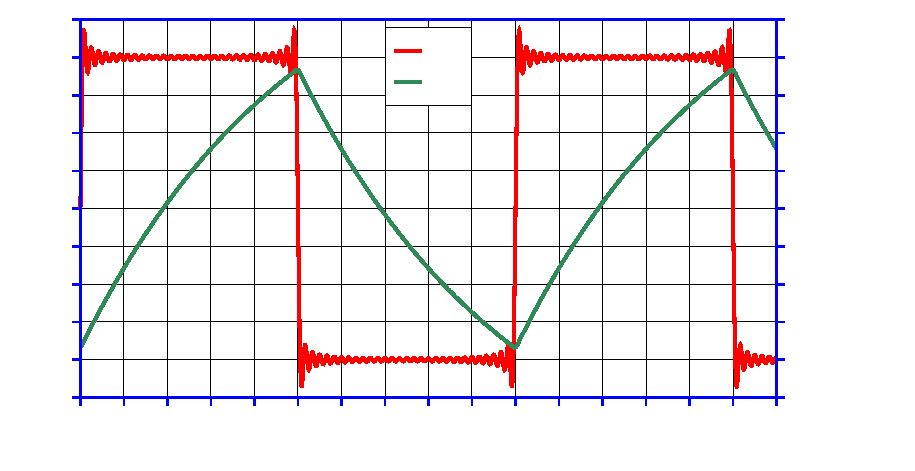
\includegraphics{Cap-Fourier-Exemple-Tensio-Corrent}}%
    \gplfronttext
  \end{picture}%
\endgroup
